\chapter{Introduction}
\section{Reasons for measuring the differential Z boson cross section}
\section{Production of dark matter at supercolliders}
In the pursuit of new physics at the CERN LHC, many scenarios have been proposed in which production of
particles that leave no trace in collider detectors
is accompanied also by production of a standard model (SM) particle, which balances the transverse momentum in an event.
The final state considered in this analysis is the production of a pair of leptons ($\ell^{+}\ell^{-}$, where $\ell=\Pe$ or $\Pgm$),
consistent with originating from a $\PZ$ boson, together with large missing transverse momentum ($\met$).
This final state is well-suited to probe such beyond the SM (BSM) scenarios, as
it has relatively small and precisely known SM backgrounds.

One of the most significant puzzles in modern physics is the nature of dark matter (DM).
In the culmination of over a century of observations, the ``$\Lambda_{\mathrm{CDM}}$'' standard model of cosmology
has established that, in the total cosmic energy budget,
known matter only accounts for about 5\%, DM corresponds to 27\%, and the rest is dark energy~\cite{2013ApJS..208...19H}.
Although several astrophysical observations indicate that DM exists and interacts gravitationally with known matter,
there is no evidence yet for nongravitational interactions between DM and SM particles.
While the nature of DM remains a mystery, there are a number of models that predict a particle physics origin. 
If DM particles exist, they can possibly be produced directly from, annihilate into, or scatter off SM particles.
Recent DM searches have exploited various methods including direct~\cite{Cushman:2013zza} and indirect~\cite{Buckley:2013bha} detection.
If DM can be observed in direct detection experiments,
it must have substantial couplings to quarks and/or gluons, and could also be produced at the LHC~\cite{Beltran:2010ww,Goodman:2010yf,Bai:2010hh,Goodman:2010ku,Fox:2011pm,Rajaraman:2011wf}.

A promising possibility is that DM may take the form of weakly interacting massive particles.
The study presented here considers one possible mechanism for producing such particles at the LHC~\cite{Abercrombie:2015wmb}.
In this scenario, a $\PZ$ boson, produced in proton-proton (pp) collisions, recoils against a pair of DM particles, $\chi\overline\chi$. The $\PZ$ boson subsequently decays into
two charged leptons, producing a low-background dilepton signature, together with $\met$
due to the undetected DM particles. In this analysis, the DM particle $\chi$ is assumed to be a Dirac fermion.
Four simplified models of DM production via an $s$-channel mediator exchange are considered.
In these models, the mediator has a spin of 1 (0) and vector or axial-vector (scalar or pseudoscalar) couplings to quarks and DM particles.
The free parameters of each model are the masses $m_{\rm med}$ and $m_{\rm DM}$ of the mediator and DM particle, respectively, as well as the coupling
constant $g_{\Pq}$ ($g_{\rm DM}$) between the mediator and the quarks (DM particles).
The vector coupling model can be described with the following Lagrangian:

\begin{equation*}
\mathcal{L}_{\text{vector}} = g_{\rm DM} {Z'}_{\mu}\overline{\chi}\gamma^{\mu}\chi  + g_{\Pq} \sum_{\Pq} {Z'}_{\mu} \overline{\Pq}\gamma^{\mu}\Pq,
\end{equation*}

\noindent where the spin-1 mediator is denoted as $\PZ'$ and the SM quark fields are referred to as \PQq and $\overline{\PQq}$.
The Lagrangian for an axial-vector coupling is obtained by making the replacement $\gamma^\mu\rightarrow\gamma^5\gamma^\mu$.
In the case of a spin-0 mediator $\phi$, the couplings between mediator and quarks are assumed to be Yukawa-like, with $g_{\Pq}$ acting as a 
multiplicative modifier for the SM Yukawa coupling ${y_{\Pq} = \sqrt{2}m_{\Pq}/v}$ (where $v = 246 \GeV$ is the SM Higgs field vacuum expectation value),
leading to the Lagrangian:

\begin{equation*}
\mathcal{L}_{\text{scalar}} = g_{\rm DM} {\phi}\overline{\chi}\chi  + g_{\Pq} \frac{\phi}{\sqrt{2}}\sum_{\Pq} y_{\Pq} \overline{\Pq}\Pq.
\end{equation*}

\noindent The Lagrangian with pseudoscalar couplings is obtained by inserting a factor of $i\gamma^5$ into each of the two terms (i.e., $\bar\chi\chi \to i\bar\chi\gamma^5\chi$ and $\bar \Pq \Pq \to i\bar \Pq\gamma^5 \Pq$). Example diagrams of DM production via spin-1 and spin-0 mediators are shown in Fig.~\ref{fig:Feynman} (upper left and right, respectively).

\begin{figure}[!hbtp]
  \centering
    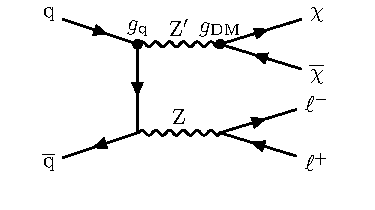
\includegraphics[width=0.45\textwidth]{figures/dmSimpFeynman.pdf}
    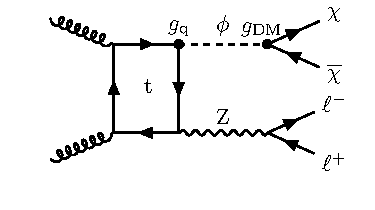
\includegraphics[width=0.45\textwidth]{figures/dmSimpFeynman_spin0.pdf}
    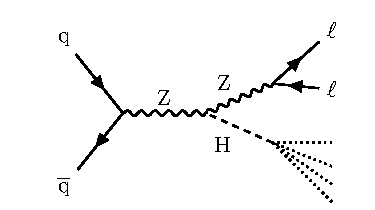
\includegraphics[width=0.45\textwidth]{figures/higgsInvisibleFeynman.pdf}
    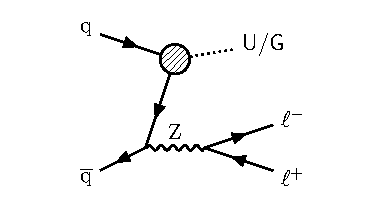
\includegraphics[width=0.45\textwidth]{figures/graph_UG.pdf}
  \caption{Feynman diagrams illustrative of the processes beyond the SM considered in this paper:
    (upper left)~DM production in a simplified model with a spin-1 mediator $\PZ'$;
    (upper right)~DM production in a simplified model with a spin-0 mediator $\phi$;
    (lower left)~production of a Higgs boson in association with Z boson with subsequent decay of the Higgs boson into invisible particles;
    (lower right)~unparticle or graviton production. The diagrams were drawn using the {\sc TikZ-Feynman} package~\cite{Ellis:2016jkw}.
  } 
      \label{fig:Feynman}
\end{figure}

A primary focus of the LHC physics program after the discovery of a Higgs boson (H)~\cite{AtlasPaperCombination,CMSPaperCombination,Chatrchyan:2013lba} by
the ATLAS and CMS Collaborations is the study of the properties of this new particle. The observation of a sizable branching
fraction of the Higgs boson to invisible states~\cite{Ghosh:2012ep,Martin:1999qf,Bai:2011wz} would be a strong sign
of BSM physics.  Supersymmetric (SUSY) models embodying R-parity conservation contain a stable neutral lightest SUSY
particle (LSP), e.g., the lightest neutralino~\cite{Belanger:2001am}, leading to the possibility of decays of the Higgs boson into pairs of LSPs.
Certain models with extra spatial dimensions predict graviscalars that could mix with the
Higgs boson~\cite{Giudice:2000av}.  As a consequence, the Higgs boson could oscillate
to a graviscalar and disappear from the SM brane. The signature would be
equivalent to an invisible decay of the Higgs boson. There could also be contributions
from Higgs boson decays into graviscalars~\cite{Battaglia:2004js}.
Similar to the simplified DM models presented earlier, ``Higgs portal'' models~\cite{Baek:2012se,Djouadi:2011aa,Djouadi:2012zc} construct a generic connection between SM and DM particles via a Higgs boson mediator.
This analysis considers decays into invisible particles of an SM-like Higgs boson produced in association with a $\PZ$ boson, as shown in Fig.~\ref{fig:Feynman} (lower left).

Another popular BSM paradigm considered here is the Arkani-Hamed--Dimopoulos--Dvali (ADD) model with large extra spatial dimensions~\cite{ArkaniHamed:1998rs,ArkaniHamed:1998nn,Han:1998sg}, which
is motivated by the hierarchy problem, i.e., the disparity between the electroweak unification
scale ($M_\mathrm{EW} \sim 1\TeV$) and the Planck scale ($M_\mathrm{Pl} \sim 10^{16}\TeV$).
This model predicts graviton (\cPG) production via the process $\PQq\PAQq \rightarrow \PZ + \cPG$. The graviton escapes
detection, leading to a mono-$\PZ$ signature (Fig.~\ref{fig:Feynman}, lower right).
In the ADD model, the apparent Planck scale in four space-time dimensions
is given by $M_\mathrm{Pl}^2 \approx M_\mathrm{D}^{n+2}R^n$, where $M_\mathrm{D}$ is the true Planck scale of
the full $n$+4 dimensional space-time and $R$ is the compactification radius of the extra
dimensions. Assuming $M_\mathrm{D}$ is of the same order as $M_\mathrm{EW}$, the observed large value
of $M_\mathrm{Pl}$ points to an $R$ of order 1 mm to 1 fm for 2 to 7 extra dimensions. The consequence of
the large compactification scale is that the mass spectrum of the Kaluza--Klein graviton states
becomes nearly continuous, resulting in a broad $\PZ$ boson transverse momentum (\PT) spectrum.

The final BSM model considered in this analysis is the phenomenologically interesting concept of unparticles, which appear in the low-energy limit of conformal field theories.
In the high-energy regime, a new, scale invariant Banks--Zaks field with a nontrivial infrared fixed point is introduced~\cite{Banks:1981nn}.
The interaction between the SM and Banks--Zaks sectors is mediated by particles of large mass scale $M_{\textsf{U}}$, below which the interaction is suppressed and can be treated
via an effective field theory (EFT). The low-energy regime will include unparticles, which have phase space factors equivalent to those of a noninteger
number of ordinary particles~\cite{Kang:2014cia,Rinaldi:2014gha,Cheng:1988zx}. In this analysis, the emission of spin-0 unparticles from SM quarks is considered.
Because of the weakness of the unparticle interactions with the SM fields, the unparticle evades detection.
The EFT Lagrangian used to interpret the results is defined as follows:

\begin{equation*}
\mathcal{L}_{U}  = \frac{\lambda}{\LU^{\dU-1}} \mathcal{O}_{\textsf{U}} \overline{\PQq}\PQq,
\end{equation*}

\noindent where $\lambda$ represents the coupling between the SM and unparticle fields, \LU is the cutoff scale of the EFT, and \dU is the characteristic scaling dimension of the theory.
The unparticle operator is denoted as $\mathcal{O}_{\textsf{U}}$.
A representative Feynman diagram of the interaction is shown in Fig.~\ref{fig:Feynman} (lower right).


